\usetikzlibrary{arrows,shapes,automata,petri,positioning}

\tikzset{
    placeyellow/.style={
        circle,
        thick,
        draw=yellow!75,
        fill=yellow!20,
        minimum size=6mm,
    },
    place/.style={
        circle,
        thick,
        draw=blue!75,
        fill=blue!20,
        minimum size=6mm,
    },
    transitionH/.style={
        rectangle,
        thick,
        fill=black,
        minimum width=8mm,
        inner ysep=2pt
    },
    transitionV/.style={
        rectangle,
        thick,
        fill=black,
        minimum height=8mm,
        inner xsep=2pt
    },
    transitionVgreen/.style={
        rectangle,
        thick,
        fill=green!60,
        minimum height=8mm,
        inner xsep=2pt
    },
    transitionVred/.style={
        rectangle,
        thick,
        fill=red!75,
        minimum height=8mm,
        inner xsep=2pt
    },
    transitionVdgreen/.style={
        rectangle,
        thick,
        fill=green!75,
        minimum height=8mm,
        inner xsep=2pt
    }
}


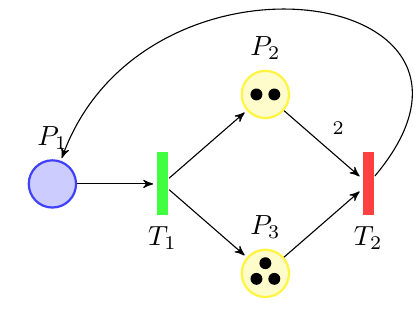
\begin{tikzpicture}[node distance=0.5cm and 1cm,>=stealth',bend angle=45,auto]
    \node [place,label=above:$P_1$] (p1) {};
    \node [transitionVdgreen,label=below:$T_1$] (t1) [right= of p1] {}
        edge[pre]   (p1);
    \node [placeyellow,tokens=2,label=above:$P_2$] (p2) [above right=of t1] {}
        edge[pre]   (t1);
    \node [placeyellow,tokens=3,label=above:$P_3$] (p3) [below right=of t1] {}
        edge[pre]   (t1);
    \node [transitionVred,label=below:$T_2$] (t2) [above right=of p3] {}
        edge[pre] node[swap]{\scriptsize 2} (p2)
        edge[pre]   (p3)
        edge[post,out=50,in=70,looseness=2,overlay]  (p1);
\end{tikzpicture}


